

\documentclass[journal,transmag]{IEEEtran}

% *** GRAPHICS RELATED PACKAGES ***
%
\ifCLASSINFOpdf
  \usepackage[pdftex]{graphicx}
  % declare the path(s) where your graphic files are
  % \graphicspath{{../pdf/}{../jpeg/}}
  % and their extensions so you won't have to specify these with
  % every instance of \includegraphics
  % \DeclareGraphicsExtensions{.pdf,.jpeg,.png}
\else
  % or other class option (dvipsone, dvipdf, if not using dvips). graphicx
  % will default to the driver specified in the system graphics.cfg if no
  % driver is specified.
  % \usepackage[dvips]{graphicx}
  % declare the path(s) where your graphic files are
  % \graphicspath{{../eps/}}
  % and their extensions so you won't have to specify these with
  % every instance of \includegraphics
  % \DeclareGraphicsExtensions{.eps}
\fi

% *** PACKAGES ***
%
\usepackage{amsmath}
%\usepackage{algorithmic}
%\usepackage{array}
%\ifCLASSOPTIONcompsoc
%  \usepackage[caption=false,font=normalsize,labelfont=sf,textfont=sf]{subfig}
%\else
%  \usepackage[caption=false,font=footnotesize]{subfig}
%\fi
%\usepackage{fixltx2e}
%\usepackage{stfloats}
% \usepackage{dblfloatfix}
%\ifCLASSOPTIONcaptionsoff
%  \usepackage[nomarkers]{endfloat}
% \let\MYoriglatexcaption\caption
% \renewcommand{\caption}[2][\relax]{\MYoriglatexcaption[#2]{#2}}
%\fi
%\usepackage{url}


% correct bad hyphenation here
\hyphenation{op-tical net-works semi-conduc-tor}


\begin{document}

\title{TCP Measurements}

\author{\IEEEauthorblockN{Jiri Hamberg}
\IEEEauthorblockA{Department of Computer Science,
University of Helsinki}}
%\thanks{Manuscript received December 1, 2012; revised August 26, 2015. 
%Corresponding author: M. Shell (email: http://www.michaelshell.org/contact.html).}}

\markboth{Network Measurement Seminar,~University of Helsinki,~2016}%
{Shell \MakeLowercase{\textit{et al.}}: Bare Demo of IEEEtran.cls for IEEE Transactions on Magnetics Journals}

\IEEEtitleabstractindextext{%
\begin{abstract}
This is the abstract. Motivation, background, topic, methodology and results are each briefly discussed here.
\end{abstract}

\begin{IEEEkeywords}
TCP, Network Measurement
\end{IEEEkeywords}}


\maketitle
\IEEEdisplaynontitleabstractindextext
\IEEEpeerreviewmaketitle

\section{Introduction}
\IEEEPARstart{T}{his} the introduction. Motivation, history and the current state of the research is discussed here. Relevance of the research topic is highlighted.

Here be a claim backed up by the some evidence~\cite{Allman99}.
Another claim backed up by more evidence~\cite{Ningning03}.

\section{Metrics and Parameters}
TCP measurements, like all network measurements, can be roughly divided to two categories: active measurements and passive measurements. In general, passive measurements aim at understanding and profiling a network without affecting it. Active measurements, on the other hand, try to capture useful information about the state of the network to enhance and adapt the network to changing circumstances.   

Passive measurements are used to evaluate the performance of the TCP protocol. One fundamental difficulty in making robust TCP measurements, is the great number of variables that may affect a measurement. Different link layer technologies, the charasteristics of the data being transmitted and the level of competing traffic, amongst other things, have been shown to have a significant impact on the behaviour of the TCP traffic~\cite{Allman99}. To draw general conclusions from an experiment, we usually need to measure some performance metric of a particular TCP version over varying network conditions~\cite{Allman99}.  

Often the goal of a TCP measurement is to compare the performance of different versions or extensions against each other. This further increases the number of parameters and the dimensionality of the measurement space of the experiment.

The variable that we are mostly interested in measuring is the RTT (round trip time) of TCP segments. In active measurements, we can extract knowledge about the state of the network by observing RTTs of consecutive segments. We will go through the details in section three. 

When making passive measurements, a metric must be chosen that represents the overall performance of the system that we are evaluating. The metric function is an aggregate value of multiple measurements over a period of time. A somewhat natural choice is the throughput of the system, meaning the total amount of data transmitted over a normalized period of time. Usually, a better alternative to throughput is goodput, which only takes into account the total amount of transmitted payload. 

The goodput alone cannot be taken as a performance metric. Consider a scenario where there are three peers and a single server in the network. Each peer tries to upload a continuous stream of data to the server taking up the maximum capacity of the bottleneck link. In a set up \textit{A}, each peer sends 100 megabits of data over 30 seconds. In a set up \textit{B}, one of the peers sends 303 megabytes of data over 30 seconds, and the other two peers are unable to send any data. Now, only considering the goodput, set up \textit{B} is clearly better, having goodput of $10.1Mb/s$, whereas set up \textit{A} only achieves goodput of $10.0Mb/s$. Clearly set up \textit{A} is the more desirable because of its \textit{fairness}.

There are quite a few possible ways to formalize the idea of fairness, but one reasonable choice is the formulation by Jain et al.~\cite{Jain84}. Given $n$ users and resource allocation schema $ \textbf{x} = (x_1,~x_2,~..,~x_n)$ (where $x_i$ is the the size of the allocation given to user $i$), the fairness measure $f(\textbf{x})$ of the schema is then given by

\begin{equation}
f(\textbf{x}) = \frac{ \left(\sum\limits_{i=1}^{n} x_i\right)^2 }{n \sum\limits_{i=1}^{n} x_i^2 } \label{fairness}
\end{equation}

The fairness measure~\eqref{fairness} has the following properties~\cite{Jain84}:
\begin{enumerate}
	\item \textbf{Scale independence}: The unit of measurement does not affect the metric.
	\item \textbf{Boundedness}:  The metric is bound between 0 (totally unfair) and 1 (totally fair).
	\item \textbf{Continuity}: Even a slight change in the allocation schema shows in the metric.  
\end{enumerate}   

A good performance measure of a TCP experiment should take both the goodput and the fairness into account. Sometimes other quantities are used as part of the metric, including segment loss rate, which indicates aggressiveness of the protocol, router queue lengths or the burstiness of connections~\cite{Allman99}. 

 
%Discussion about measuring techniques and variables to measure. Distinction between active and passive measurements. Aggregate measurements. How to evaluate TCP performance; metrics to consider:

%\begin{enumerate}
%	\item Throughput/Goodput
%	\item Fairness
%	\item Loss rate
%\end{enumerate}

%\section{Active Measurements}
%Measurements that affect the decisions made by a node in the network. TCP itself relies on active measurements, such as tracking RTT:s of segments.

\section{Improving TCP Startup Performance with Active Measurements}

We will now demonstrate how active measurements can be used to improve the TCP startup algorithm. We will closely follow the work of Ningning Hu and P. Steenkiste~\cite{Hu03} in introducing the \textit{paced start} algorithm, a proposed replacement for the \textit{slow start} algorithm.

In TCP slow start, the congestion window size is exponentially increased until a packet is lost or the congestion window size reaches a predefined value of \textit{ssthresh}, in order to find out a suitable congestion window size. This often results either a fairly conservative bandwidth estimate or considerable number of lost packets. The packet stream emitted by the algorithm is also quite bursty, which may cause load spikes in the router queues of the network. The load spikes increase packet losses of other connections in the network~\cite{Hu03}.    

In paced start algorithm, a bandwidth estimation method called PTR (Packet Transmission Rate)~\cite{Hu03b} is used to estimate the available bandwidth of the path during the TCP startup. In the PTR method, the source machine sends a sequence of packet trains, starting with a tiny inter-packet-gap in the initial packet train. The average inter-packet-gap of the ACK-packet-trains from the target machine will be measured. The source machine will repeatedly adjust its inter-packet-gap based on the measured inter-packet-gap of the target machine, and keep sending new packet trains, until its inter-packet-gap equals the measured inter-packet-gap of the target machine. At this point, the source machine and the target machine are processing packages at approximately the same rate. This rate will give the estimate for the available bandwidth on the path~\cite{Hu03b}. The error of bandwidth estimates given by the PTR algorithm is in most cases smaller than 30\%~\cite{Hu03b}, which is comparable to the error in bandwidth estimates given by slow start.   

\begin{figure}
	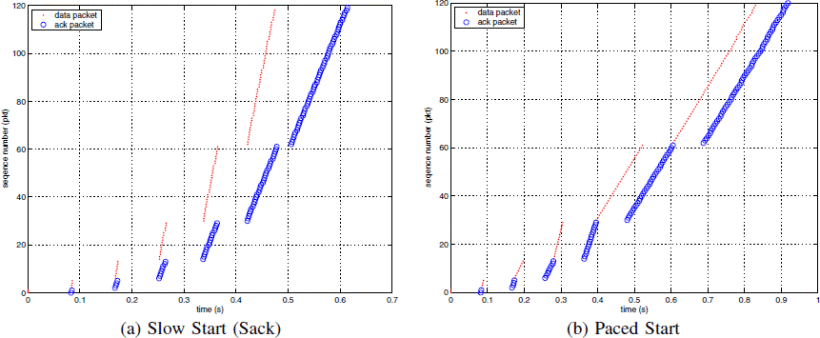
\includegraphics[width=0.5\textwidth]{images/hu03_PTR.png}
	\caption{Figure by Hu et al.~\cite{Hu03}. Packet trains of source and target machines plotted against time for both slow start and paced start algorithm. The data is from a simulation with roundtrip time of 80ms, a bottleneck link of 5Mb/s and available bandwidth of 3Mb/s. In plot (b), the difference of the inter-packet-gaps of the packet trains from source and the target machines converges, yielding the estimate for the available bandwidth. This convergence is visualised in the slopes of the blue and red lines becoming equal.}
	\label{fig:PTR}
\end{figure}
The paced start algorithm is based on the insight, that the TCP startup, with minor changes, can be viewed as a sequence of packet trains, making the PTR method applicable~\cite{Hu03}. The paced start algorithm has two major differences to the slow start algorithm. First, the paced start algorithm is not self clocking (arrival of an ACK does not trigger the sending of packages), because in a self clocking setup the sent and received packets are not even close to being evenly paced, making the inter-packet-gap meaningless to measure. Instead, the paced start only sends a new packet train after the previous packet train has been entirely acknowledged. This allows us to distinguish the packet trains from one another. 

Secondly, paced start iteratively searches for the optimal packet sending rate using the PTR method. The algorithm terminates when a packet is lost or a timeout occurs, just like slow start but also if a sufficiently good packet sending rate is found. Figure~\ref{fig:PTR}, by Ningning Hu and P. Steenkiste~\cite{Hu03}, illustrates the workings of the PTR method.

The paced start algorithm can be described as follows:
\begin{enumerate}
	\item Set \textit{source\_gap} to 0 and \textit{congestion\_window\_size} to 2.
	\item Send \textit{congestion\_window\_size} packets with \textit{source\_gap} and measure \textit{ack\_gap}
	\item Set \textit{source\_gap} to $2 \textit{ack\_gap}$
	\item Double \textit{congestion\_window\_size}, send \textit{congestion\_window\_size} packets with \textit{source\_gap} and measure \textit{ack\_gap}
	\item If packet loss or timeout occurs, start congestion avoidance
	\item If $\textit{src\_gap} - \textit{ack\_gap} \approx 0$, send \textit{congestion\_window\_size} packages and start congestion avoidance, else goto 7
	\item Adjust \textit{source\_gap} based on \textit{ack\_gap} and goto 4 
\end{enumerate} 
The adjustment to \textit{source\_gap} on step 7 is based on the binary search algorithm: if the \textit{source\_gap} is smaller than the measured \textit{ack\_gap}, then we are sending packets at a rate higher than the available rate, and the \textit{source\_gap} must be increased. New \textit{source\_gap} is set to is set to the middle point between measured \textit{ack\_gap} and current upper bound on \textit{source\_gap}.

If \textit{source\_gap} is smaller than the \textit{ack\_gap}, we are sending packets at a lower rate than what is available and the \textit{source\_gap} must be lowered. The \textit{source\_gap} is set to the middle point between previous \textit{source\_gap} and the current lower bound on \textit{source\_gap}.

Figure \ref{fig:paced_start}, by Ningning Hu and P. Steenkiste~\cite{Hu03}, illustrates the bandwidth search functionality of paced start algorithm in the two-dimensional space of sending rate (Y-axis) and train length (X-axis).

\begin{figure}
	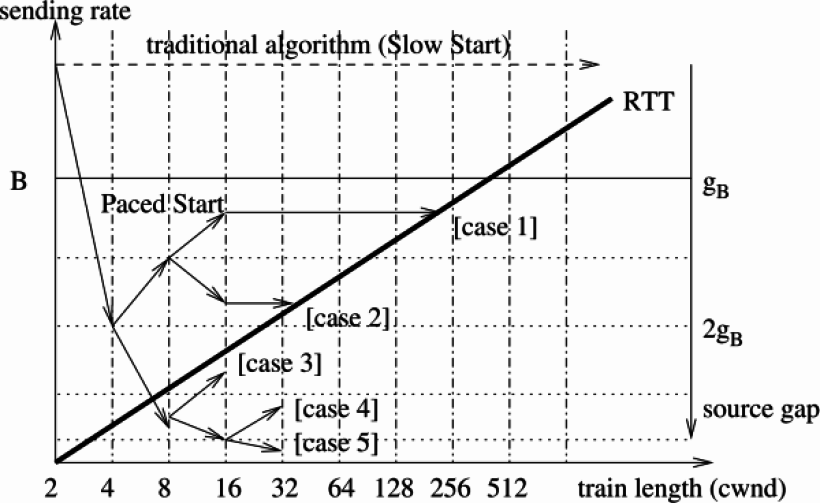
\includegraphics[width=0.5\textwidth]{images/hu03_paced_start_search.png}
	\caption{Figure by Hu et al.~\cite{Hu03}. Slow start algorithm moves along the X-axis until a suitably large cwnd is found (or ssthresh is hit). Paced start also considers the Y-axis, doing a binary search to find the suitable sending rate. Cases 1 to 5 represent possible routes that the binary search may take, depending on the ideal sending rate.}
	\label{fig:paced_start}
\end{figure}

Hu and Steenkiste used ns2 simulator~\cite{Singh12} and real system measurements to evaluate the paced start algorithm, comparing it against the slow start algorithm and TCP Vegas and TCP NewReno, both of which implement their own improvements on the TCP startup algorithm. We well omit the comparison to Vegas and NewReno here and focus solely on the comparison between slow start and paced start. We also omit the large scale network simulation here, reviewing only small scale simulations and system measurements.

Hu and Steenkiste used the following metrics: \textit{throughput} (throughput of the whole connection),  \textit{loss} (loss rate of the whole connection), \textit{su-throughput} (throughput of the startup period), \textit{su-loss} (loss rate of the startup period) and \textit{su-time} (start up period length).  

In the simulation, node \textit{A} initiates a TCP connection to node \textit{B}. The traffic goes through a path that has two routers \textit{$R_1$} and \textit{$R_2$} in between the nodes. Node \textit{A} is connected to \textit{$R_1$} by a fast low latency connection, as is \textit{B} to \textit{$R_2$}. 

The connection between \textit{$R_1$} and \textit{$R_2$} is set at 100Mbps, while the competing traffic load that goes through routers \textit{$R_1$} and \textit{$R_2$} is varied. Metrics \textit{throughput}, \textit{su-throughput}, \textit{loss} and \textit{su-time} are measured, comparing slow start to paced start. The measurements lasted for 50 seconds. Figure~\ref{fig:competing_traffic}, by Ningning Hu and P. Steenkiste~\cite{Hu03}, compiles these measurements.

The lowermost plot clearly shows that paced start moves to congestion avoidance faster than slow start in this scenario. The difference in startup times grows smaller as the amount of competing traffic increases, since slow start requires less and less round trips to find a suitable congestion window.

The plot in the middle shows that paced start algorithm did not lose any packets in this simulation while slow start's loss rate increased as a function of competing traffic. 

The uppermost plot shows that both slow start and paced start achieved roughly the same throughput over the time period of 50 seconds. Paced start performed somewhat better than slow start when little competing traffic was present. This is because in this case, the paced start is able to move to congestion avoidance much faster than slow start. 

Overall, the paced start seems to perform very well compared to slow start in this setup: it is clearly less aggressive, finds a suitable congestion window faster and even has a slight positive impact on the overall throughput.

\begin{figure}
	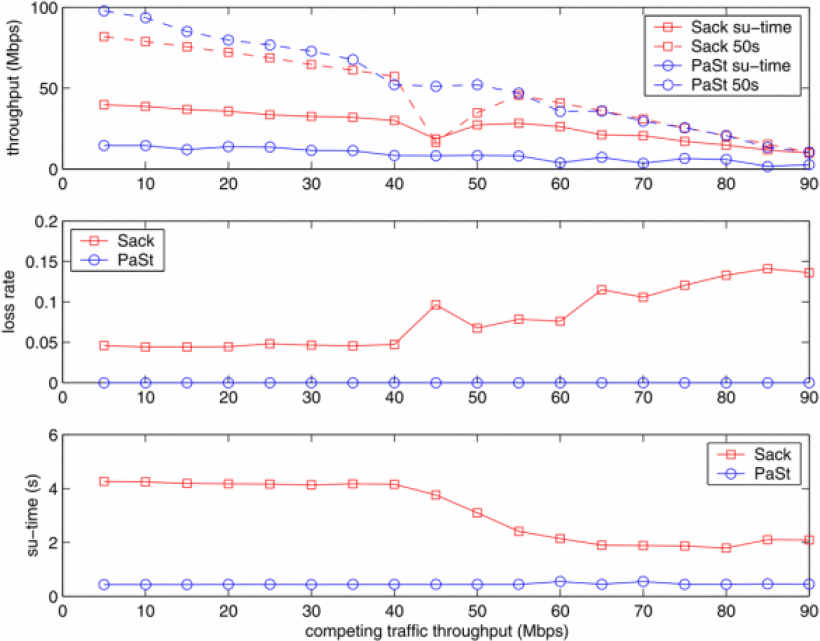
\includegraphics[width=0.5\textwidth]{images/hu03_competing_traffic.png}
	\caption{Figure by Hu et al.~\cite{Hu03}. The effect of competing traffic on the performance of slow start (Sack) and paced start (PaSt) algorithms. ns2 network simulation.}
	\label{fig:competing_traffic}
\end{figure}

A number of experiments were conducted using in-kernel implementation of paced start. The environment was a testbed on Emulab~\cite{Emulab} consisting of two Apache servers and two web request generators, one of each on each side of a bottleneck link, so that bidirectional traffic was generated over the bottleneck link. One of the web servers was configured to use the paced start -kernel while all other hosts used the slow start kernel. The experiments lasted for 500 seconds, each generating around 2100 requests. The web request generators' log files were used to calculate the throughput distribution for downloading web pages. Figure~\ref{fig:in_kernel} contains the throughput distributions, as a CDFs (cumulative distribution functions), of both Apache servers. The web server using paced start lost 1168 packets during the experiment while the web server using slow start lost 94186 packets. The trend of this experiment seems to be similar to that of the simulation: paced start seems to be outperforming slow start in both throughput and packet loss rate.

\begin{figure}
	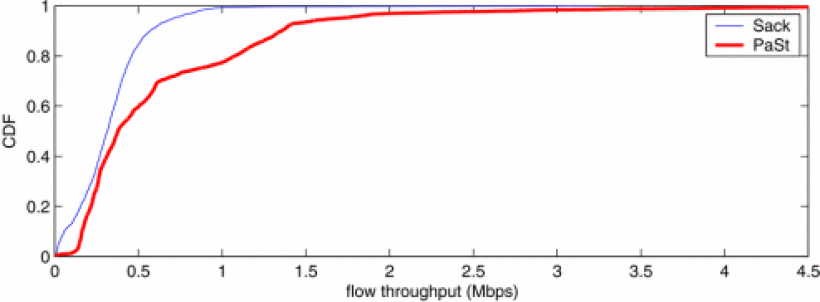
\includegraphics[width=0.5\textwidth]{images/hu03_in_kernel.png}
	\caption{Figure by Hu et al.~\cite{Hu03}. Cumulative distribution functions of flow throughput during a 500 second experiment conducted on a Emulab testbed. Paced start in red and slow start in blue.}
	\label{fig:in_kernel}
\end{figure}



%the difference between the spacing in the data packets and the acknowledgement packets is used to infer information about the bandwidth of the route.


%Alternatively this subsection could be a separate section.

\section{Passive Measurements}
One important aspect of any measurement based TCP experiment, is choosing the environment in which the experiment is to be conducted. In this section, different platforms are considered. We discus pros and cons of each platform and give a high level overview of the techniques involved.  

\subsection{Testbeds}

A testbed refers to a relatively small isolated network that is fully controlled by the conductors of the experiment~\cite{Allman99}. Testbeds provide total control of the experiment unlike live internet tests, making the experiment possibly more robust and reproducible. The main downside of a testbed is the cost: creating a complex setting with a rich topology can cost a lot of money. 

Compared to simulated settings, testbeds tend to yield more accurate results, since real systems are being tested. 

\subsection{Live Internet Tests}

Live Internet tests are experiments, where a mesh of hosts on the Internet, controlled by the experimenters, communicate with one another. There are various ways to set up such an experiment, the most complete of which is to have each of the \textit{N} hosts send data to one another, giving \textit{$O(N^2)$} different network paths to measure with~\cite{Allman99}.

In this type of experiment, the experimenters have no control over the underlying network, making it impossible to measure the effect that the generated traffic has on other traffic of the network on the same path. The main benefit of live internet tests is that they are quite simple and inexpensive to implement and they can be used to run tests in a wide variety of network conditions.

\subsection{Simulation} 

Multiple scriptable general purpose simulation frameworks, such as ns2~\cite{Singh12} exist today. Some researchers also write their specialized simulators from the ground up~\cite{Allman99}. Simulators offer a major cost and time savings compared to real world measurements~\cite{Allman99}, especially so when an experiment contains multiple parameters that must be varied. Mutating the network topology, for example, can be quite tedious in a real world setting. Another advantage is that a simulation can test TCP performance in a network that does not currently exist in real world, making it possible to predict how an algorithm may perform in the future.   

One major disadvantage posed by simulations, is that there is always a certain amount of loss of detail involved. Estimating whether or not the lost details matter to the outcome of the simulation may be difficult. Thus, results of simulations are often at least partially validated in a real world experiments.    

\subsection{Emulation}

An emulation refers to an experiment that is a mixture of a real world experiment, usually a testbed, and a simulation~\cite{Allman99}. An emulator models a part of a network path between two real nodes. As an example, emulation may be useful for modeling part a network that cannot be easily incorporated in a physical experiment, such as a satellite channel~\cite{Allman99}. This allows the researchers to isolate the simulation to only a part of the whole experiment, making the results as credible as a real world experiment, so long as the isolated simulation is reliable enough.   

%Here stuff about the different end-to-end methodologies that can be applied to measuring TCP.

%\subsection{Testbeds}
%Pros and cons of using testbeds.

%\subsection{Live Internet Tests}
%Pros and cons of using live internet tests.

%\subsection{Emulation}
%Pros and cons of using emulation.

%\section{Applications}
%Applications of the TCP measurements.

%\subsection{Evaluating Congestion Control Algorithms}
%Stuff about congestion control in Vegas, Reno and others variants of TCP.

%\subsection{Improving TCP Startup Performance}

\section{Evaluating Congestion Control Algorithms}
In this section, we will be looking at a work by I. Abdeljaouad et al.~\cite{Abdeljaouad10}, where the performance of three modern TCP variants, Cubic, Compound and New Reno, were compared using ns2 network simulator~\cite{Singh12}. We will start by quickly introducing each of the three TCP variants followed by a summary of the experiment and analysis conducted by I. Abdeljaouad et al.

\subsection{Cubic}

Cubic is the default TCP implementation of Linux kernels from version 2.6.19 onwards. The congestion window of Cubic is determined by the following function~\cite{Ha08}

\[
W_{cubic}(t) = C(t - K)^3 + W_{max}   
\]

where $C$ is a scaling factor, $t$ is the time since last congestion window reduction, $W_{max}$ is the window size before last congestion window reduction and $K = (W_{max} \beta / C)^{1 / 3}$, where $\beta$ is the fractional reduction applied to $W_{max}$ during the last reduction~\cite{Ha08}. It follows~\cite{Ha08}, that upon a window reduction, the $W_{cubic}$ first grows rapidly, but the growth slows down as the $W_{cubic}$ gets close to previous $W_{max}$. As the window grows past previous $W_{max}$, the $W_{cubic}$ starts to grow rapidly again. 

Compared to slow start, the Cubic algorithm better utilizes the knowledge gathered from previous window reduction event, reducing the amount of lost packages. As a self clocking algorithm, the slow start is also biased by RTT of a path: the smaller the RTT, the quicker the slow start grows the congestion window. Cubic on the other hand, is indifferent to the RTT of a path, making it more fair~\cite{Ha08}. 

\subsection{Compound}

Compound is a TCP variant that was introduced in Windows Vista Windows Server 2008. The Compound TCP is based on the insight that the regular TCP congestion avoidance phase is ill suited with modern high throughput networks~\cite{Tan05}. Filling the capacity of such a path may take hours, when the congestion window is only increased by one packet every RTT~\cite{Tan05}.

The Compound congestion control algorithm introduces a delay-based component to the congestion window calculations~\cite{Tan05}, during the congestion avoidance phase, while maintaining the default slow start behaviour of regular TCP. The delay based component maintains an exponentially smoothed estimate of current RTT. If the difference between the smoothed current RTT and the measured RTT exceeds a predefined constant, then early congestion is detected. The exact way in which the window size is updated for both the delay-based component and the "regular" component, is a bit technical. Their conjoined effect on the congestion window, can be expressed as follows~\cite{Tan05}:

\[
win(t + 1) = win(t) + \alpha win(t)^k
\]
when no packet loss or early congestion is detected, and
\[
win(t + 1) = win(t) * (1 - \beta)
\]
when packet loss or early congestion is detected. Here $\alpha$, $\beta$ and $k$ are configurable constants. 
  
\subsection{New Reno}

New Reno is a TCP variant based on TCP Reno~\cite{rfc6582}. Reno implements the fast recovery algorithm, in which the slow start phase is skipped in case of a fast retransmit (upon receiving a specific number of acknowledgements with the same sequence number, the sender assumes that the packet was dropped, and immediately resends), halving the current congestion window and immediately starting congestion avoidance. 

New Reno improves the fast recovery algorithm by being able to maintaining a decent flight size and not re-triggering the window reduction during multiple packet losses in a single congestion window~\cite{rfc6582}.  

\subsection{Experiment and Analysis}

The experiment conducted in \cite{Abdeljaouad10} consists of two parts: a wired and a wireless simulation. In both setups, goodput and fairness were measured with and without the presence of reverse traffic. Reverse traffic was introduced to the simulations because it increases the burstiness of the TCP by compressing the ACK messages on the reverse path~\cite{Abdeljaouad10}. 

In the wired setup, a single TCP source sends data to a TCP sink over a 2Mbps bottleneck link. The RTT of the connection is 250ms and the links between the sources and the sinks are 1Gbps. There are also 10 TCP sources on the other side of the bottleneck link, sending reverse traffic to 10 TCP sinks located on the same side of the bottleneck link as the forward traffic source. Figure~\ref{fig:topology1} shows the network topology of the wired simulation. The connection lasted for 1000 seconds and the TCP sources on the reverse path only sent data from $t=250s$ to $t=500s$ and from $t=750s$ to $t=1000s$. This setup was repeated for each of the three TCP variants. Table~\ref{tab:goodput1} collects the results obtained by  I. Abdeljaouad et al.

\begin{figure}
	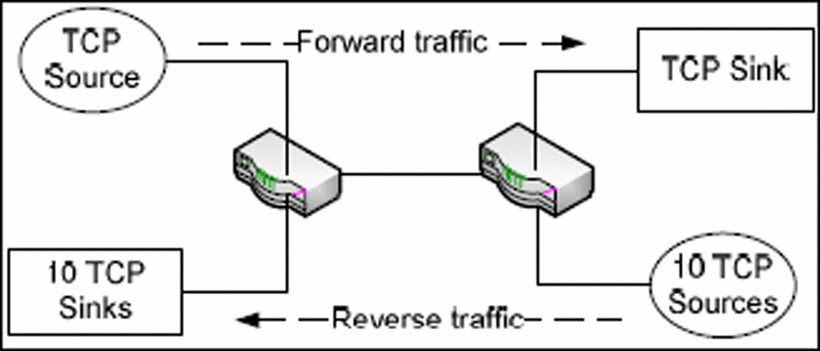
\includegraphics[width=0.5\textwidth]{images/abdeljaouad10_topology_1.png}
	\caption{Figure by I. Abdeljaouad et al.~\cite{Abdeljaouad10}. Topology of the wired ns2 network simulation.}
	\label{fig:topology1}
\end{figure}

\begin{table}
\small
\begin{tabular}{l*{3}{c}l}
& Compound & Cubic & New Reno & Rev. Traffic \\
\hline
0s-250s Mbps & 1.99 & 1.99 & 1.98 & No \\
250s-500s Mbps & 1.79 & 1.96 & 1.71 & Yes \\
500s-750s Mbps & 2.00 & 2.00 & 1.99 & No \\
750s-1000s Mbps & 1.80 & 1.96 & 1.76 & Yes \\
\end{tabular}
\caption{Based on results by I. Abdeljaouad et al.~\cite{Abdeljaouad10}. Goodput achieved by each TCP variant with and without reverse traffic at different time intervals.}
\label{tab:goodput1}
\end{table}

In this scenario, Cubic and Compound were both able to utilize the whole path capacity when no other traffic was present, both performing slightly better than New Reno. When reverse traffic was introduced, Cubic clearly outperformed Compound and New Reno, and Compound performed slightly better than New Reno.  

To measure the fairness of the TCP variants, the setup was slightly modified. Instead of one sender and one sink in the forward path, $M$ sources and sinks were simulated. Figure~\ref{fig:topology2} shows the modified network topology.

\begin{figure}
	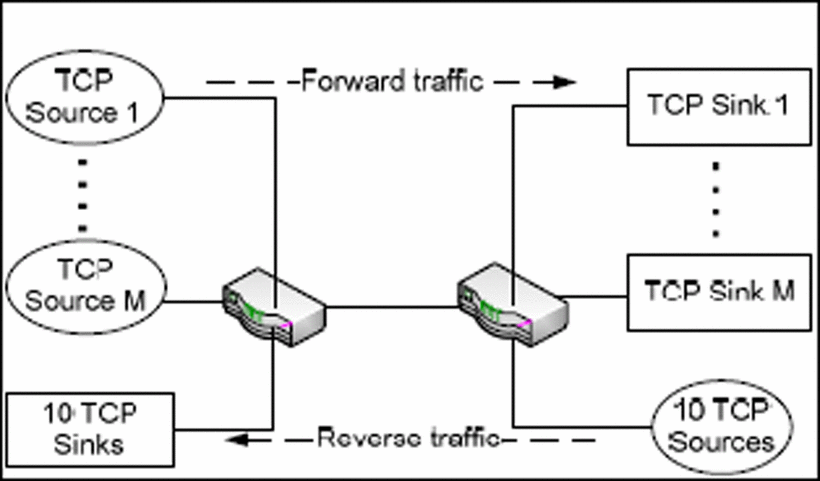
\includegraphics[width=0.5\textwidth]{images/abdeljaouad10_topology_2.png}
	\caption{Figure by I. Abdeljaouad et al.~\cite{Abdeljaouad10}. Topology of the wired ns2 network simulation to measure the fairness of the TCP variants.}
	\label{fig:topology2}
\end{figure}

The fairness was measured for each TCP variant with the number of concurrent senders, $M$, varying from 10 to 200. The RTTs of the senders were randomly selected from a uniform distribution ranging from $20 + 230/M$ to $250$ milliseconds to approximate variance in RTTs of TCP connections in real world. Figure~\ref{fig:fairness1} shows the measured fairness index~\eqref{fairness} for each TCP variant as a function of $M$.

\begin{figure}
	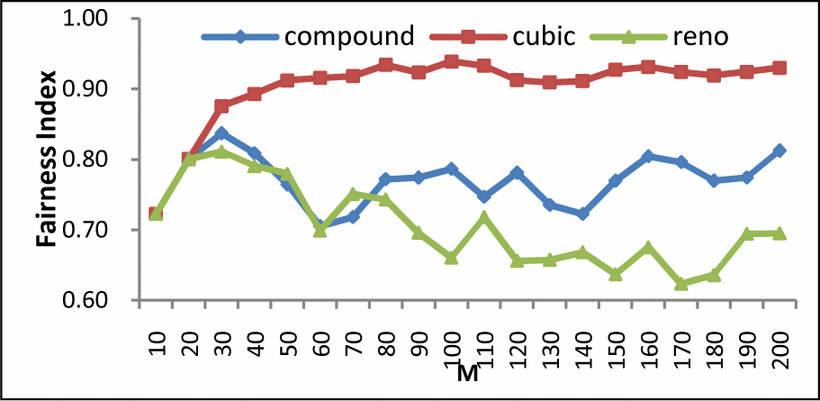
\includegraphics[width=0.5\textwidth]{images/abdeljaouad10_fairness_1.png}
	\caption{Figure by I. Abdeljaouad et al.~\cite{Abdeljaouad10}. Fairness of TCP variants as a function of concurrent senders.}
	\label{fig:fairness1}
\end{figure}

The measurements clearly show that Cubic has the highest fairness of the variants. This result is likely due to the fact that the Cubic treats connections with different RTTs equally, whereas the other variants favour connections with short RTTs. Compound seems to be somewhat fairer than New Reno when the number of concurrent connections is greater than 70. 

In the second set of simulations, the authors looked at the behaviour of the TCP variants over wireless links. The scenario was similar to the previously discussed simulations, except now the TCP sources and sinks at the end of the forward path were mobile and the wireless link was the bottleneck of the connections. All wired links were 1Gbps, while the wireless link and the mobile nodes ran the IEEE802.11g protocol at 54Mbps data rate. Figure~\ref{fig:topology3} shows the network topology of this scenario. Reverse traffic was introduced to the network similarly to the wired scenario.     

\begin{figure}
	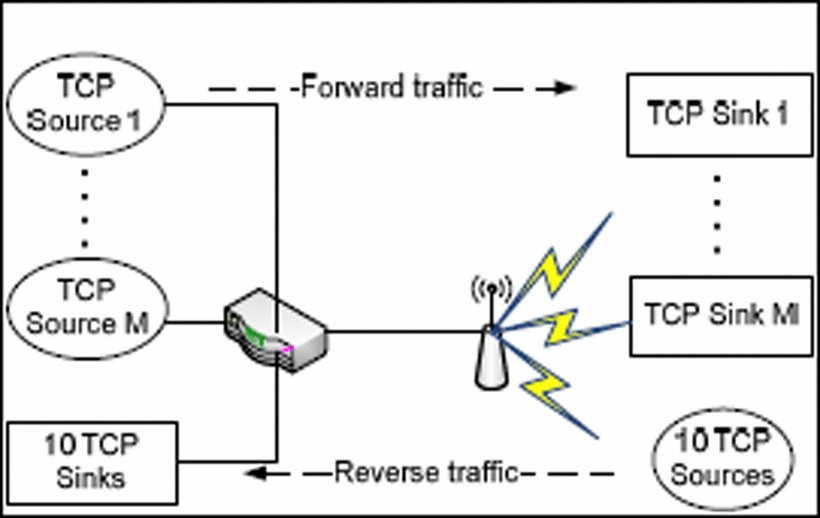
\includegraphics[width=0.5\textwidth]{images/abdeljaouad10_topology_3.png}
	\caption{Figure by I. Abdeljaouad et al.~\cite{Abdeljaouad10}. Topology of the wireless ns2 simulation.}
	\label{fig:topology3}
\end{figure}

The measurements show that New Reno outperformed Compound and Cubic in fairness. This is not surprising, since Cubic and Compound are optimized for high throughput networks~\cite{Ha08,Tan05}. Compound had the best goodput, while New Reno and Cubic had nearly identical goodput. The goodputs obtained by all the variants were quite low. The authors argue, that this is mainly due to the reverse traffic causing ACK packages to be drastically delayed, which severely hampers the performance of all three variants. Figure~\ref{fig:goodput} contains the goodputs measured for each variant as a function of concurrent connections.

\begin{figure}
	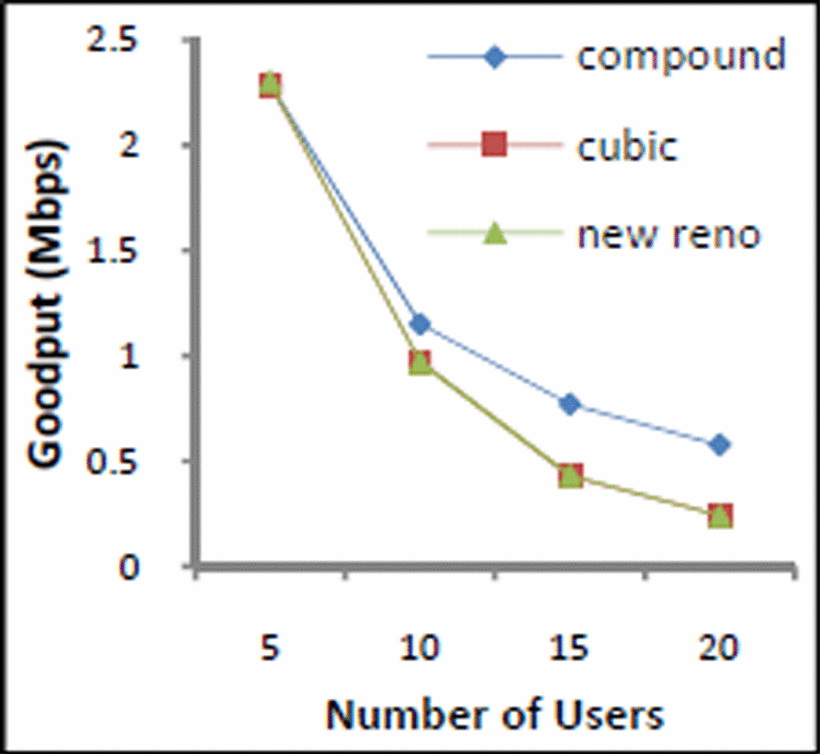
\includegraphics[width=0.5\textwidth]{images/abdeljaouad10_goodput.png}
	\caption{Figure by I. Abdeljaouad et al.~\cite{Abdeljaouad10}. Goodputs obtained by the TCP variants in the wireless ns2 simulation as a function of concurrent connections. }
	\label{fig:goodput}
\end{figure}

All the protocols achieved a good level of fairness in this setup, New Reno being fairest by a clear margin and Cubic performing slightly better than Compound. Figure~\ref{fig:fairness2} contains the fairness~\eqref{fairness} measured for each variant as a function of concurrent connections.

\begin{figure}
	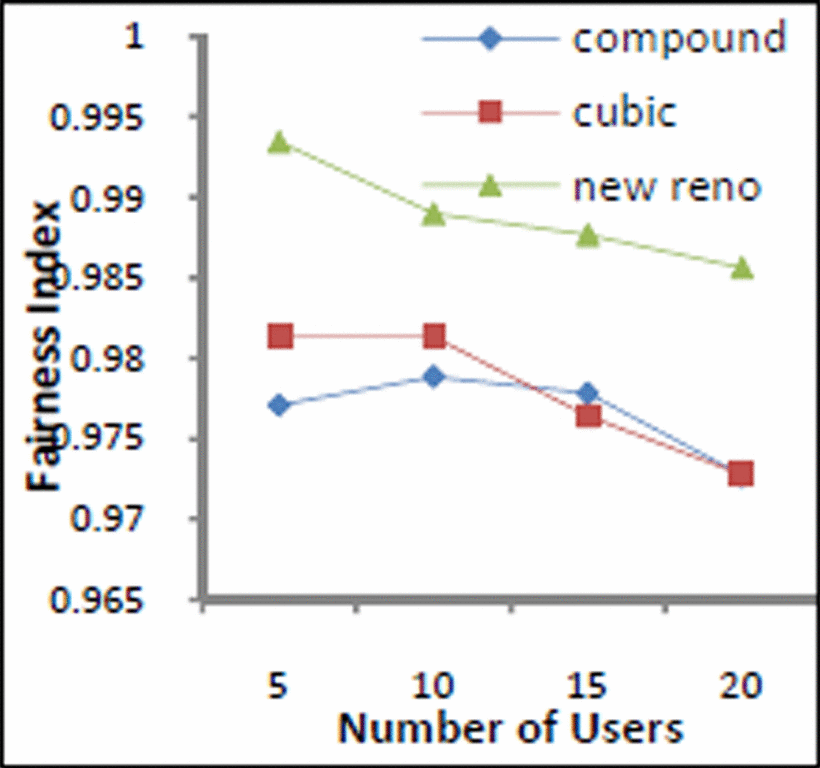
\includegraphics[width=0.5\textwidth]{images/abdeljaouad10_fairness_2.png}
	\caption{Figure by I. Abdeljaouad et al.~\cite{Abdeljaouad10}. Fairness index measured for the TCP variants in the wireless ns2 simulation as a function of concurrent connections.}
	\label{fig:fairness2}
\end{figure}

\section{Conclusion}
The conclusion goes here.


%\appendices
%\section{Proof of the First Zonklar Equation}
%Appendix one text goes here.

% you can choose not to have a title for an appendix
% if you want by leaving the argument blank


%\section*{Acknowledgment}
%The authors would like to thank...

\ifCLASSOPTIONcaptionsoff
  \newpage
\fi


%\begin{thebibliography}{1}

%\bibitem{IEEEhowto:kopka}
%H.~Kopka and P.~W. Daly, \emph{A Guide to \LaTeX}, 3rd~ed.\hskip 1em plus
%  0.5em minus 0.4em\relax Harlow, England: Addison-Wesley, 1999.
%\end{thebibliography}

\bibliographystyle{IEEEtran}
\bibliography{references}


%\begin{IEEEbiographynophoto}{Jiri Hamberg}
%Biography text here.
%\end{IEEEbiographynophoto}

\end{document}

